\chapter{Resultados e discussões}
\label{chap:resultados}

Com o resultado desse trabalho, a comunidade acadêmica passa a dispor e utilizar um sistema web chamado Mercado Universitário que facilita o fluxo de mercância. A interface idealizada do sistema foi alcançada em sua maior parte, bem como a disponibilização do código fonte.

O sistema proposto foi desenvolvido de acordo com seus diagramas e requisitos apresentados na seção \ref{chap:etapas_desenvolvimento}. Buscou-se fazer um sistema bonito, intuitivo e robusto para que \textit{queries} ao banco de dados fossem pouco custosas para que o servidor não ficasse sobrecarregado devido as consultadas simultâneas dos usuários.

Divulgado para o público no dia 13 de janeiro de 2020 por meio de redes sociais, o sistema foi calorosamente acolhido pelas pessoas que compõem o âmbito universitário. O link de acesso para o trabalho desenvolvido é \url{http://www.mercadouniversitario.com}, onde será possível realizar o cadastro público para ter acesso aos produtos comercializados, bem como criar uma conta de vendedor para assim divulgar algum produto ao qual deseja-se vender.

\section{Apresentando a aplicação}

Nessa seção iremos apresentar as telas do sistema que apresentam as principais funcionalidades do trabalho.
% Também iremos apontar se os requisitos funcionais e objetivos foram alcançados da forma esperada.
Através do sistema foi possível alcançar os objetivos propostos.

% Através do sistema foi possível alcançar os objetivos propostos. Entre eles, a listagem de produtos foi alcançada através da interface vista na Figura XXX, ai podemos ver que os produtos são listados -----, organizados através de filtros -----, 
% A parte de avaliação do vendedor foi possível através da interface proposta na Figura XXX, alí podemos ver -----

% \subsection{Objetivo Geral}
% Propor uma aplicação gratuita de \textit{e-commerce} C2C(\textit{Consumer to Consumer}), voltada para o comércio informal na Universidade Estadual de Santa Cruz.

% \subsection{Objetivos Específicos}
% O atual projeto tem alguns objetivos específicos, são eles:
% \begin{enumerate}
%     \item Criar mecanismos para o gerenciamento e compartilhamento de produtos à venda;
%     \item Possibilitar a listagem de produtos por filtros;
%     \item Permitir aos compradores fazerem pedidos de produtos;
%     \item Desenvolver interfaces para avaliação dos usuários;
%     \item Validar o sistema por meio de testes automatizados;
%     \item Disponibilizar o código fonte do sistema.
% \end{enumerate}

Na Figura \ref{fig:login} é apresentada a tela de login da aplicação, onde será possível criar uma nova sessão no sistema para que assim seja possível visualizar os produtos e vendedores da universidade do usuário logado. Por meio dessa tela existe fácil acesso a uma página de cadastro e de recuperação de senha da aplicação.

A parte de listagem de produtos foi possível através da interface proposta na Figura \ref{fig:produtos}, os produtos são listados apresentando sua fotos, nome e valor correspondente de cada produto, tal listagem pode estar filtrada de várias formas diferentes, são elas: palavra-chave, categoria, vendedor ou campus de uma universidade.

Por meio da interface proposta na Figura \ref{fig:produto} é apresenta a tela de um produto em específico. Nessa tela é possível ter todas as informações disponibilizadas pelo vendedor para esse produto, informações essas que são: foto, nome, descrição, categoria e preço. Por meio dessa tela também é possível realizar a inserção do produto em questão na lista de pedidos, se faz necessário apenas definir a quantidade do produto e clicar no botão.

\begin{figure}[htbp!]
  \centering
  \caption{Tela de login}
  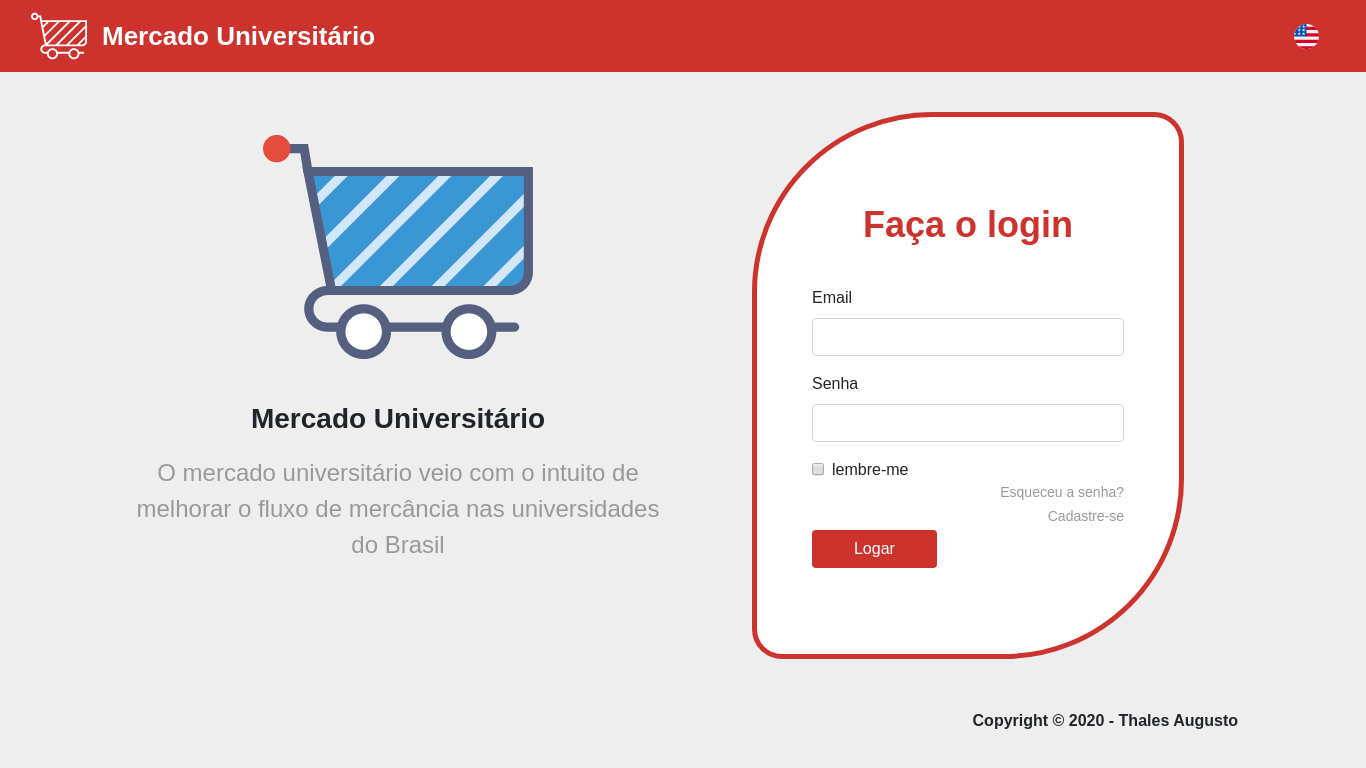
\includegraphics[width=1\textwidth]{figs/resultado/login.png}
    \legend{Fonte: Elaborada pelo autor.}
    \label{fig:login}
\end{figure}

\begin{figure}[htbp!]
  \centering
  \caption{Tela de produtos}
  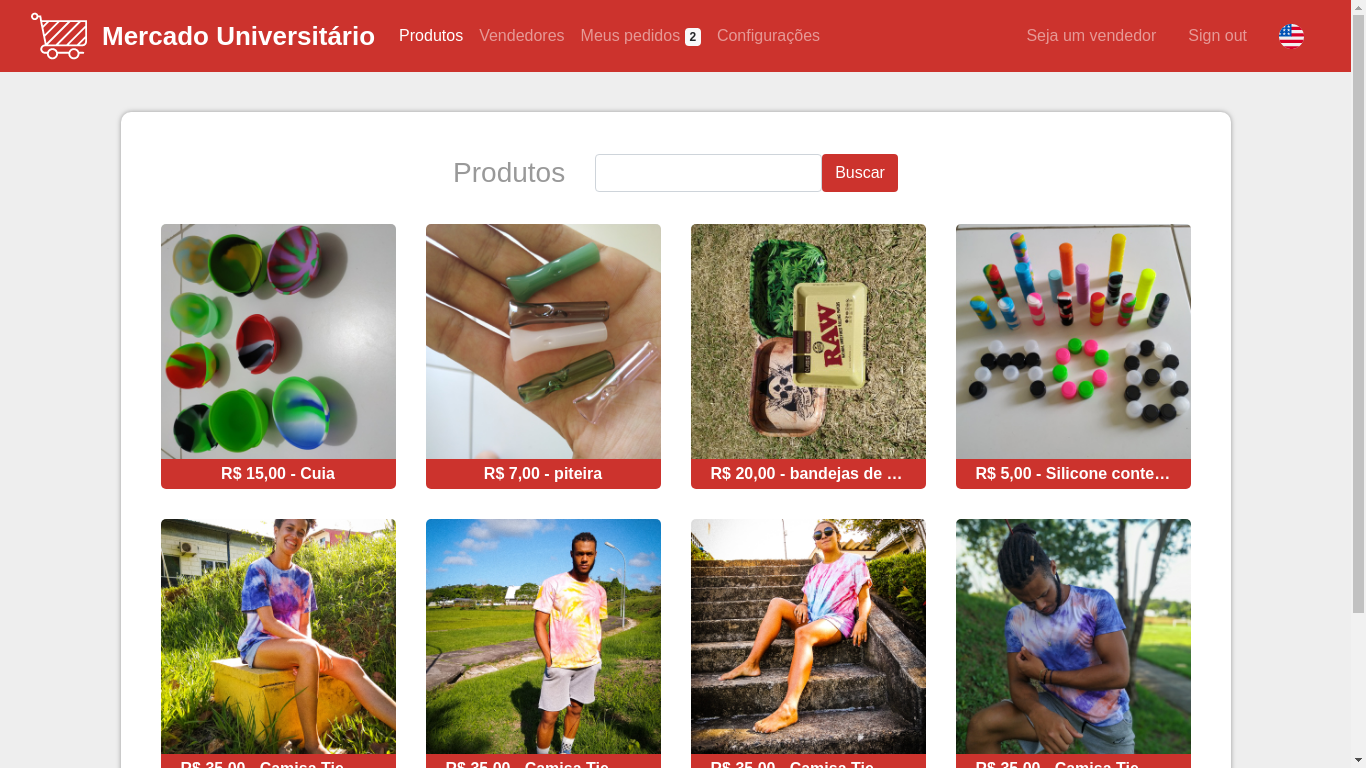
\includegraphics[width=1\textwidth]{figs/resultado/produtos.png}
    \legend{Fonte: Elaborada pelo autor.}
    \label{fig:produtos}
\end{figure}

A criação de uma página individual do vendedor foi alcançada através da interface vista na Figura \ref{fig:vendedor}, nessa tela pode ser visualizadas todas informações declaradas pelo vendedor em questão e seus clientes, como: foto de perfil, avaliações dos clientes(com nota e texto), descrição, meios para contato(Instagram e Whatsapp), se atualmente está em funcionamento e se realiza entrega. Essa tela tem fácil acesso a lista de produtos desse mesmo vendedor.

\begin{figure}[htbp!]
  \centering
  \caption{Tela individual do produto}
  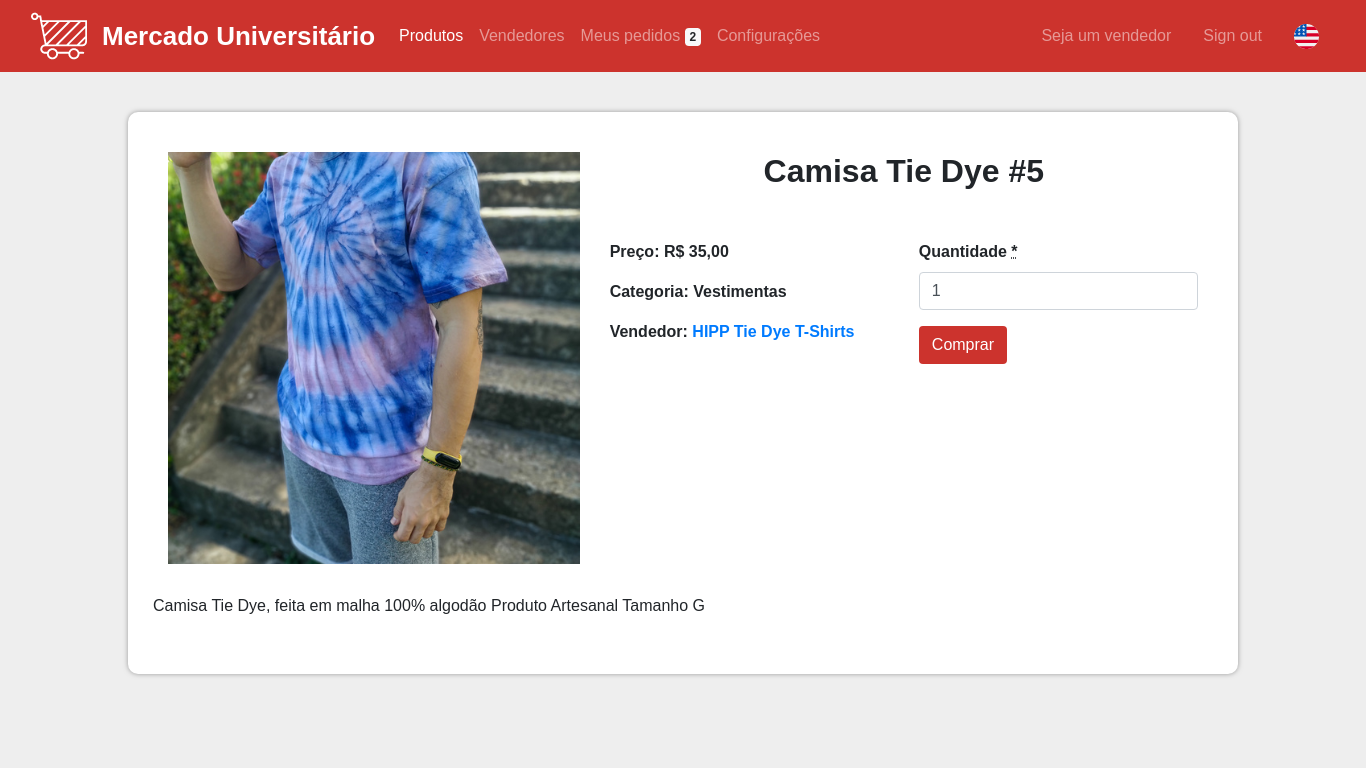
\includegraphics[width=1\textwidth]{figs/resultado/produto.png}
    \legend{Fonte: Elaborada pelo autor.}
    \label{fig:produto}
\end{figure}

Por meio da interface proposta na Figura \ref{fig:pedidos} foi possível alcançar o resultado esperado. A tela lista os pedidos(realizados e pendentes) detalhando cada produto de cada pedido mostrando seu valor individual e total da compra. Nessa tela é possível facilmente realizar um novo pedido para o vendedor deixando uma nota para que o cliente possa requisitar algo específico para o vendedor nessa compra, bem como definir um local de entrega caso o vendedor realize entrega. Caso o cliente desista de realizar a compra, ele pode cancelar rapidamente.

\begin{figure}[htbp!]
  \centering
  \caption{Tela de individual do vendedor}
  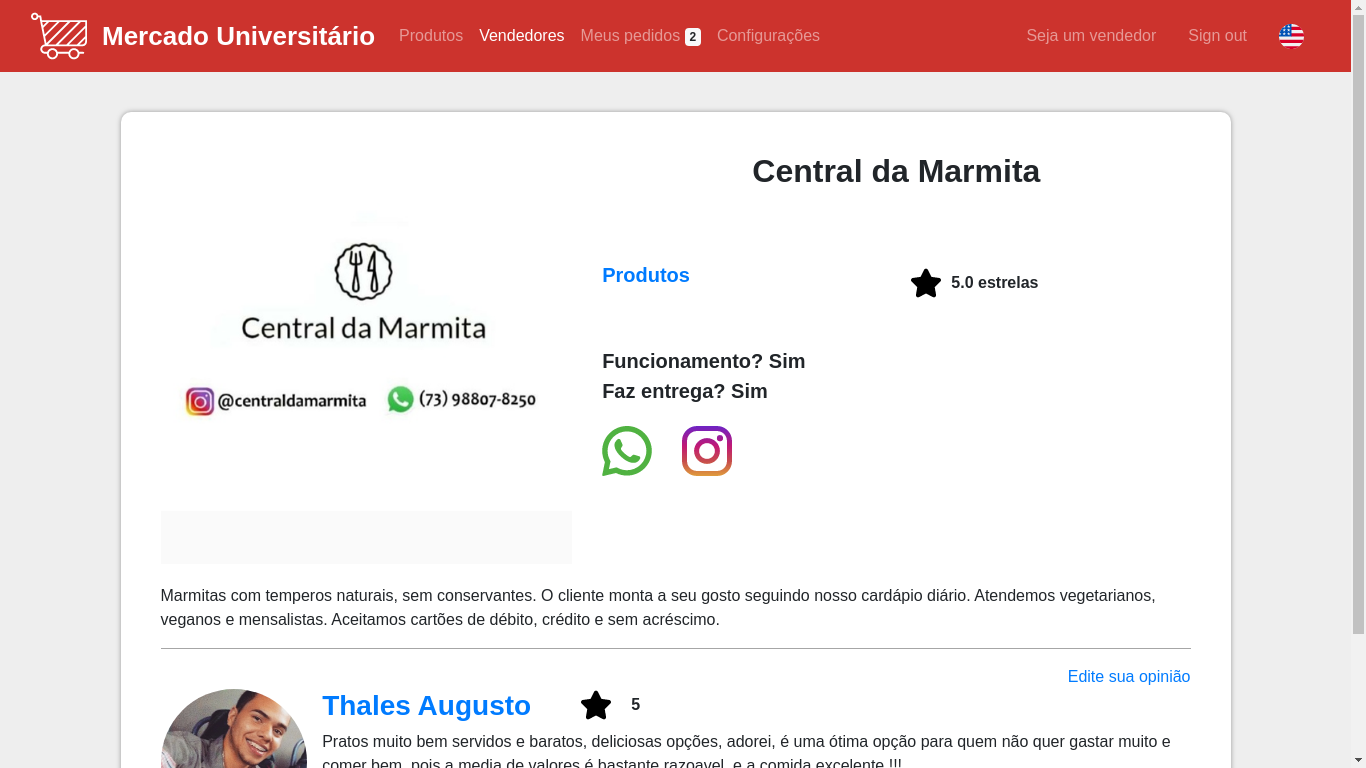
\includegraphics[width=1\textwidth]{figs/resultado/vendedor.png}
    \legend{Fonte: Elaborada pelo autor.}
    \label{fig:vendedor}
\end{figure}

\begin{figure}[htbp!]
  \centering
  \caption{Tela de pedidos}
  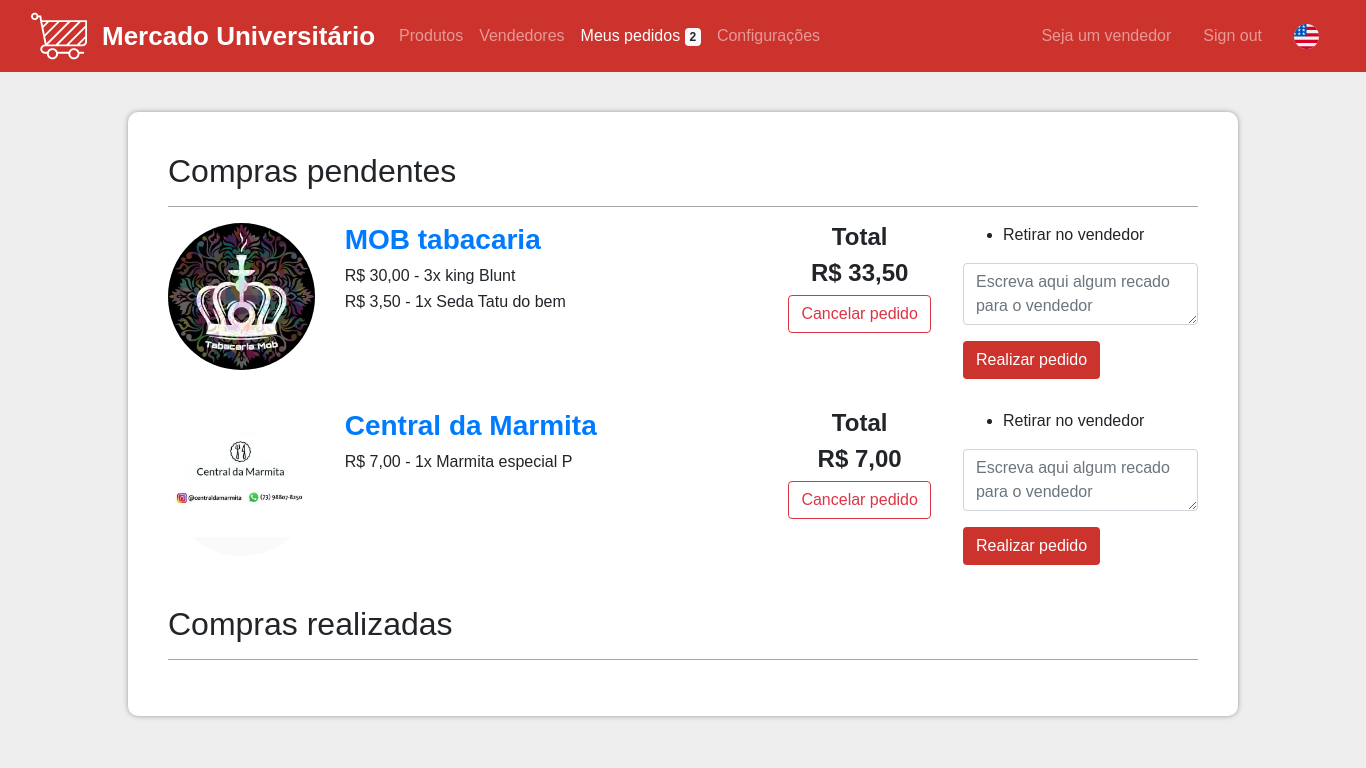
\includegraphics[width=1\textwidth]{figs/resultado/carrinho.png}
    \legend{Fonte: Elaborada pelo autor.}
    \label{fig:pedidos}
\end{figure}

\clearpage
\section{Comparação com projetos correlatos}

A proposta de valor do Mercado Universitário se assemelha muito a do Mercado Livre, pois tem como premissa o acesso a um grande número de consumidores e acesso a um grande número de produtos em um ambiente confiável. Por outro lado, o Mercado Universitário se assemelha bastante ao OLX pelo seu segmento de cliente, já que nessa plataforma é implementado um sistema de e-commerce C2C, outro ponto de semelhança é a ausência do meio de pagamento diretamente na plataforma.

Diante disso, o Mercado Universitário foi desenvolvido de acordo com suas necessidades específicas para seu nicho e buscando unir as melhores características de cada plataforma estudada como trabalhos correlatos.

\section{Validação do sistema}

Como citado na seção \ref{section:tdd}, foi utilizado a técnica TDD para desenvolvimento do trabalho, dessa forma foi possível validar o sistema implementado por meio de testes automatizados. A assertividade desses testes serão demonstrados aqui nesta seção e poderá ser confirmada por qualquer pessoa que deseja, pois o código fonte de toda aplicação está disponível no Github por meio do link \url{https://github.com/tarv7/mercado-universitario}.

Foi avaliada de forma sistemática toda a implementação técnica desenvolvida até o momento, buscando-se uma melhor eficiência e qualidade do código da aplicação. Serão realizados quatro tipos de testes automatizados no Mercado Universitário. Testes unitários e integração, testes de segurança e testes de qualidade do código, tais testes serão apresentados a seguir.

\subsection{Testes unitários e integração}

Foi utilizada a gem RSpec para esse tipo de teste. Tal ferramenta foi apresentada na seção \ref{rspec}. De acordo com a Figura \ref{fig:rspec} foram realizados 101 exemplos de testes na aplicação, tais testes conseguiram cobrir 91.66\% de todo o código da   aplicação sem que ocorresse nenhuma falha. Tal resultado se mostra bastante satisfatório, uma vez que se aproxima bastante de 100\% de cobertura do código e não apresenta nenhuma falha.

\begin{figure}[htbp!]
  \centering
  \caption{Saída do terminal para teste automatizado unitário e de integração juntos utilizando a \textit{gem} RSpec}
  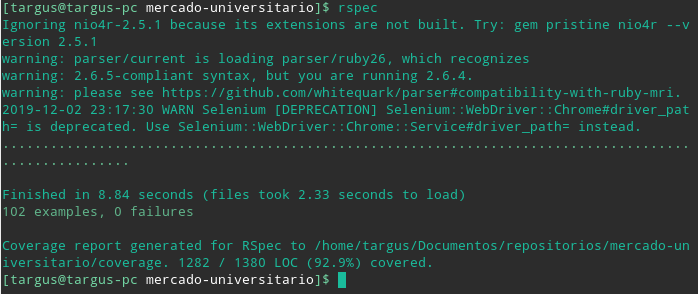
\includegraphics[width=1\textwidth]{figs/rspec.png}
    \legend{Fonte: Elaborada pelo autor.}
    \label{fig:rspec}
\end{figure}


\subsection{Testes de segurança}

Foram utilizadas duas \textit{gems} para realizar esse teste de grande importância para a aplicação. A \textit{gem} Brakeman em conjunto com a \textit{gem} Bundle Audit são suficientes para explorar as principais vulnerabilidades das aplicações web. Como é observado nas imagens \ref{fig:brakeman} e \ref{fig:audit}, não foram encontradas nenhuma vulnerabilidade na aplicação.


\subsection{Testes de qualidade do código}

Para ser possível garantir uma boa manutenção e legibilidade futura do código, foi necessário utilizar a \textit{gem} Rubocop(apresentada na seção \ref{rubocop}). Como observado na Figura \ref{fig:rubocop}, foram verificadas as boas práticas de programação determinadas pelo Rails em 71 arquivos do trabalho, não foi encontrada nenhuma ofensa no código.

\begin{figure}[htbp!]
  \centering
  \caption{Saída do terminal para teste automatizado de segurança utilizando a \textit{gem} Brakeman}
  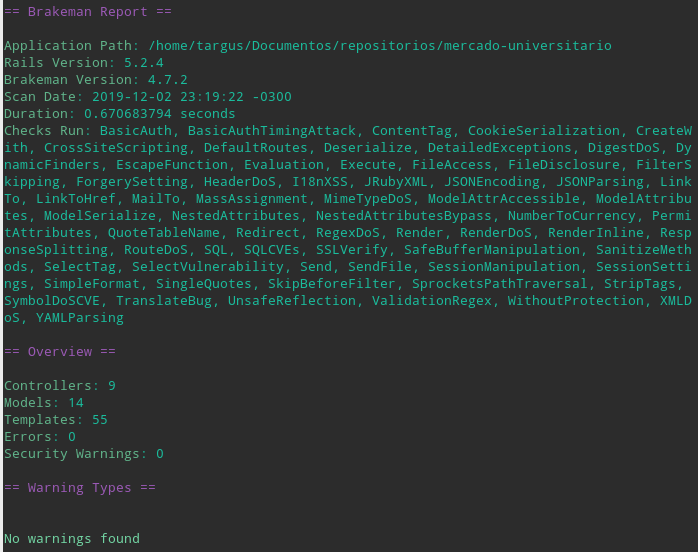
\includegraphics[width=1\textwidth]{figs/brakeman.png}
    \legend{Fonte: Elaborada pelo autor.}
    \label{fig:brakeman}
\end{figure}

\begin{figure}[htbp!]
  \centering
  \caption{Saída do terminal para teste automatizado de segurança utilizando a \textit{gem} Bundle Audit}
  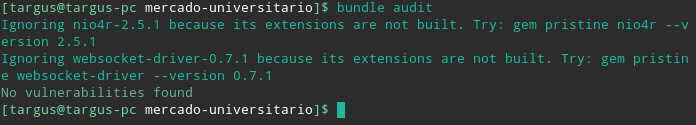
\includegraphics[width=1\textwidth]{figs/bundle_audit.png}
    \legend{Fonte: Elaborada pelo autor.}
    \label{fig:audit}
\end{figure}

\clearpage
\begin{figure}[h]
  \centering
  \caption{Saída do terminal para verificação da qualidade do código utilizando a gem Rubocop}
  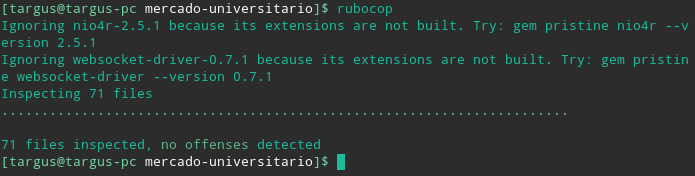
\includegraphics[width=1\textwidth]{figs/rubocop.png}
    \legend{Fonte: Elaborada pelo autor.}
    \label{fig:rubocop}
\end{figure}
